% --------------------------------------------------------------
% This is all preamble stuff that you don't have to worry about.
% Head down to where it says "Start here"
% --------------------------------------------------------------
 
\documentclass[12pt]{article}
 
\usepackage[margin=1in]{geometry} 
\usepackage{amsmath,amsthm,amssymb}
\usepackage{graphicx}
\usepackage{soul}
\usepackage[utf8]{inputenc}
\usepackage[french]{babel}

\usepackage{url}
\usepackage{hyperref}
\hypersetup{
    colorlinks=true,
    linkcolor=blue,
    filecolor=magenta,      
    urlcolor=cyan,
    }
\newcommand{\N}{\mathbb{N}}
\newcommand{\Z}{\mathbb{Z}}

\usepackage{xcolor}
\newcommand{\red}[1]{{\color{red}#1}}
 
\newenvironment{theorem}[2][Theorem]{\begin{trivlist}
\item[\hskip \labelsep {\bfseries #1}\hskip \labelsep {\bfseries #2.}]}{\end{trivlist}}
\newenvironment{lemma}[2][Lemma]{\begin{trivlist}
\item[\hskip \labelsep {\bfseries #1}\hskip \labelsep {\bfseries #2.}]}{\end{trivlist}}
\newenvironment{exercise}[2][Exercise]{\begin{trivlist}
\item[\hskip \labelsep {\bfseries #1}\hskip \labelsep {\bfseries #2.}]}{\end{trivlist}}
\newenvironment{reflection}[2][Reflection]{\begin{trivlist}
\item[\hskip \labelsep {\bfseries #1}\hskip \labelsep {\bfseries #2.}]}{\end{trivlist}}
\newenvironment{proposition}[2][Proposition]{\begin{trivlist}
\item[\hskip \labelsep {\bfseries #1}\hskip \labelsep {\bfseries #2.}]}{\end{trivlist}}
\newenvironment{corollary}[2][Corollary]{\begin{trivlist}
\item[\hskip \labelsep {\bfseries #1}\hskip \labelsep {\bfseries #2.}]}{\end{trivlist}}
 
\begin{document}
 
% --------------------------------------------------------------
%                         Start here
% --------------------------------------------------------------
 
%\renewcommand{\qedsymbol}{\filledbox}
 
\title{Compétition Kaggle 1 IFT 6390/3395}
 
\maketitle

\section{Introduction}
\label{sec:intro}

% TODO: color href: https://www.overleaf.com/learn/latex/Hyperlinks
Pour ce projet, vous participerez à une compétition Kaggle sur la détection de chiffres manuscrits. L'objectif est de concevoir un algorithme d'apprentissage qui peut classer automatiquement des images. La figure \ref{fig:my_label} montre un exemple d'image provenant du jeu de données d'entraînement. Toutes les images (y compris ceux du jeu de données de test retenus) sont de dimension $56\times28$. La classe d'une image est indiquée par la somme de ces chiffres. Par exemple, la classe de l'image de la figure \ref{fig:my_label} est 10. Nous avons généré ce jeu des données à partir de MNIST. L'ensemble d'entraînement et l'ensemble de test pour ces données se composent respectivement de 50 000 et 10 000 échantillons. 
\begin{figure}[h]
    \centering
    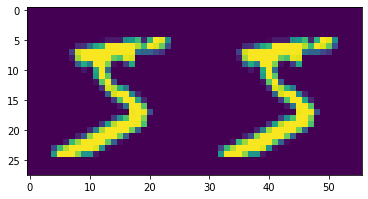
\includegraphics[width=0.5\linewidth]{figures/img1.png} 
    
    \caption{Exemple d'image du jeu de données d'entraînement}
    \label{fig:my_label}
\end{figure}
Vous devez implémenter et entraîner plusieurs algorithmes de classification basés sur le jeu de données fourni. L'évaluation sera basée sur la performance sur le jeu de test fourni et sur un rapport écrit.

La compétition, y compris les données, est disponible ici : 

\begin{center}
\href{https://www.kaggle.com/t/0d0b1c033ece47ffa1dbc8bd374689ae}{https://www.kaggle.com/t/0d0b1c033ece47ffa1dbc8bd374689ae}
\end{center}

\section{Dates importantes et information}
\label{sec:dates}

Veuillez prendre en considération les échéances importantes suivantes :
 
% À FAIRE : confirmer les dates
\begin{itemize}
   \item \textbf{5 octobre 23\!:59} Date de publication du concours
  \item \textbf{12 octobre 23\!:59} Date limite pour s'inscrire à la compétition sur Kaggle.
  \item \textbf{26 octobre 23\!:59} Fin du concours. Plus aucune soumission Kaggle n'est autorisée.
  \item \textbf{3 novembre 23\!:59} Les rapports et le code sont dûs sur Gradescope.
\end{itemize} 
 
\textbf{Note sur le partage et le plagiat} :
Vous êtes autorisé à discuter des techniques générales avec les autres équipes. Vous n'êtes PAS autorisé à partager votre code. Ce comportement constitue du plagiat et il est très facile à détecter. Toutes les équipes impliquées dans le partage de code recevront une note de 0 dans la compétition de données.

\section{Participation à la compétition et formation de l'équipe} 

Les étudiants de \textbf{IFT3395} travailleront en équipe de 2 ou 3. Les étudiants de \textbf{IFT6390A/B} doivent faire la compétition seul. 

\subsection{Formation d'une équipe Kaggle (étudiants IFT3395 uniquement)}

Pour former une équipe:
\begin{itemize}
\item Inscrivez-vous à la compétition et créez un compte Kaggle si vous n'en avez pas déjà, en suivant ce lien: \href{https://www.kaggle.com/t/0d0b1c033ece47ffa1dbc8bd374689ae}{https://www.kaggle.com/t/0d0b1c033ece47ffa1dbc8bd374689ae}
\item Dans l'onglet ``Invite Others", ajoutez les noms de vos coéquipiers.
\item Vos coéquipiers vont maintenant devoir accepter l'invitation.
\item Remplissez le formulaire google \url{https://forms.gle/Jrscpc5p6ee3x9Vw7} avec les membres de votre équipe avant le \textbf{12 octobre à 23:59}. Toutes équipes qui ne se sont pas inscrites ou qui se sont inscrites après la date limite ne seront pas évaluées.
\end{itemize}

\textbf{Important:} Le nombre maximum de soumissions par jour et par équipe est de 2, et par ÉQUIPE. Si au moment de la formation d'une équipe le total des soumissions par les membres est plus que 2, il ne sera pas possible de créer l'équipe ce jour-ci.
Par exemple: C'est le premier jour de la compétition. Les étudiants A,B,C veulent former une équipe.
\begin{itemize}
    \item A a soumis 0 fois.
    \item B a soumis 2 fois.
    \item C a soumis 1 fois.
\end{itemize}
Le maximum autorisé est de 2 évaluations par jour et par équipe, mais la somme des évaluations des futurs membres de l'équipe est déjà de 3. Par conséquent, ils ne pourront pas former une équipe aujourd'hui, et ils devront attendre demain.

Vous pouvez cependant effectuer des évaluations avant de former une équipe, tant que vous prenez bien en compte la limite au jour de la création de l'équipe.



\section{Bases de référence}
\label{sec:baselines}

% A FAIRE : les élèves voient-ils une régression logistique ?
% À FAIRE : ajouter des lignes de base à la compétition Kaggle
Nous vous demandons de créer un classificateur \textbf{régression logistique} et de battre les bases de référence mises en évidence dans le classement. Ces bases de référence sont :

\begin{itemize}
    \item un classificateur fictif qui prédit simplement la classe la plus fréquente dans le jeu de données d'entraînement.
    \item un classificateur de régression logistique.
    \item la meilleure base de référence de l'auxiliaire d’enseignement.
\end{itemize}

Pour participer au concours, vous devez fournir une liste de  prédictions pour les instances sur le site web de Kaggle. Vous pouvez soumettre 2 prédictions par jour au cours de la compétition. Nous vous suggérons donc de commencer tôt, en vous accordant suffisamment de temps pour soumettre plusieurs fois et avoir une idée de vos performances.

Pour chacune des 3 bases de référence que vous battez, vous obtenez des points supplémentaires.

Votre classificateur de régression logistique doit être implémenté à partir de zéro. En dehors des bibliothèques Python standard, les seules bibliothèques autorisées sont \texttt{numpy}, les matrices creuses de scipy (\texttt{scipy.sparse}) et \texttt{pandas}. 

\section{Autres modèles}
 
Vous devez essayer au moins \textbf{1 autre modèle} en plus de la régression logistique, et comparer leurs performances. Vous êtes encouragés à essayer les techniques étudiées pendant le cours et à rechercher d'autres moyens de résoudre cette tâche. Voici quelques idées:

\begin{itemize}
    \item Machine à vecteurs de support
    \item Na\"ive Bayes
    \item Forêts aléatoires
    \item Utiliser des features fait-mains qui prennent en compte la nature des données
\end{itemize}

L'objectif est de concevoir la méthode la plus performante telle que mesurée en soumettant des prédictions pour l'ensemble de test sur Kaggle. Votre performance finale sur Kaggle comptera comme critère d'évaluation (voir Section \ref{sec:report}). Si un modèle testé ne fonctionne pas bien, vous pouvez toujours l'ajouter dans votre rapport et expliquer pourquoi vous pensez qu'il n'est pas approprié pour cette tâche. Ce type de discussion est un élément important que nous utiliserons pour évaluer votre rapport final de concours.

Pour cette partie, vous êtes libre d'utiliser n'importe quelle bibliothèque de votre choix. 

\section{Rapport}
\label{sec:report}

En plus de vos méthodes, vous devez rédiger un rapport qui détaille les techniques de pré-traitement, de validation, d'algorithmique et d'optimisation, ainsi que des résultats qui vous aident à comparer différentes méthodes/modèles.

Le rapport doit contenir les sections et éléments suivants :

\begin{itemize}
  \item Titre du projet
  \item Nom de l'équipe sur Kaggle, ainsi que la liste des membres de l'équipe, y compris leurs noms complet et leurs matricules.
  \item Introduction: décrivez brièvement le problème et résumez votre approche et vos résultats.
  \item Feature Design: Décrivez et justifiez vos méthodes de pré-traitement, et comment vous avez conçu et sélectionné vos features.
  \item Algorithmes: donnez un aperçu des algorithmes d'apprentissage utilisés sans entrer dans trop de détails, sauf si nécessaire pour comprendre d'autres détails.
  \item Méthodologie: inclure toutes les décisions concernant la division de l'ensemble d'entrainement et de validation, les stratégies de régularisation, les astuces d'optimisation, le choix des hyper-paramètres, etc.
  \item Résultats: présentez une analyse détaillée de vos résultats, y compris des graphiques et des tableaux. Cette analyse doit être plus large que le simple résultat de Kaggle: inclure une courte comparaison des hyper-paramètres les plus importants et de toutes les méthodes (au moins 2) que vous avez essayé.
  \item Discussion: discutez des avantages/inconvénients de votre approche et de votre méthodologie et proposez des idées d'amélioration.
  \item Division des contributions: décrire brièvement les contributions de chaque membre de l'équipe vers chacune des composantes du projet (par exemple, définir le problème, développer la méthodologie, coder la solution, effectuer l'analyse des données, rédiger le rapport, etc.) À la fin de l'énoncé des contributions, ajouter la mention suivante : ``Nous déclarons par la présente que tous les travaux présentés dans ce rapport sont ceux des auteurs''.
  \item Références: très important si vous utilisez des idées et des méthodes que vous avez trouvées dans un papier ou en ligne; c'est une question d'intégrité académique.
  \item Annexe (facultatif): Ici, vous pouvez inclure des résultats supplémentaires, plus de détails sur les méthodes, etc.
  \end{itemize} 
  
Vous perdrez des points si vous ne suivez pas ces directives. \textbf{Le texte principal du rapport ne doit pas dépasser 6 pages.} Les références et annexes peuvent dépasser les 6 pages.
%Le format doit
%be colonne unique, police 10pt, min. 1 marges. Vous pouvez utiliser la norme
% Format de conférence %IEEE, par ex. https://www.ieee.org/conferences
%events/conferences/publishing/templates.html

% À FAIRE : confirmer les données
Vous devez soumettre votre rapport et votre code sur Gradescope avant le \textbf{3 novembre 23\!\!:59}.

\subsection*{Instructions de soumission}
 
\begin{itemize}
\item Vous devez soumettre le code développé pendant le projet.
Le code doit être bien documenté.
Le code doit inclure un fichier README contenant des instructions sur
comment exécuter le code.
\item Le fichier de prédiction contenant vos prédictions sur l'ensemble de test doit être soumis en ligne sur le site Web de Kaggle.
\item Le rapport au format pdf~(écrit selon les critères définit au-dessus) et le code doivent être téléchargés sur Gradescope.
\end{itemize} 


\section{Critères d'évaluation}


Les notes seront attribuées en fonction des critères suivants :

\begin{enumerate}
     \item Des points vous seront attribués pour chacune des 3 bases de référence que vous battez.
     \item Des points vous seront attribués en fonction de votre performance finale à la fin de la compétition, donnée par votre classement par rapport à la classe.
     \item Des points vous seront attribués en fonction de la qualité et de la solidité technique de votre rapport final (voir ci-dessus).
\end{enumerate} 

% \subsection*{Evaluation of the report}

% For the written report, the evaluation criteria include:
% \begin{itemize}
% \item Technical soundness of the methodology (pre-processing, feature selection,
% validation, algorithms, optimization).
% \item Technical correctness of the description of the algorithms (may be
% validated with the submitted code).
% \item Meaningful analysis of final and intermediate results.
% \item Clarity of descriptions, plots, figures, tables.
% \item Organization and writing. Please use a spell-checker and do not underestimate
% the power of a well-written report!!
% \end{itemize}
% Do note that the grading of the report will place emphasis on the quality
% of the implemented classifiers as well as the rationale
% behind the pre-processing and optimization techniques. The code should be
% clear enough to reflect the logic articulated in the report. We are looking
% for a combination of insight and clarity when grading the reports.

\end{document}
